\section{Method: \ours{}}
\label{sec:method}

\begin{figure*}[t]
  \centering
  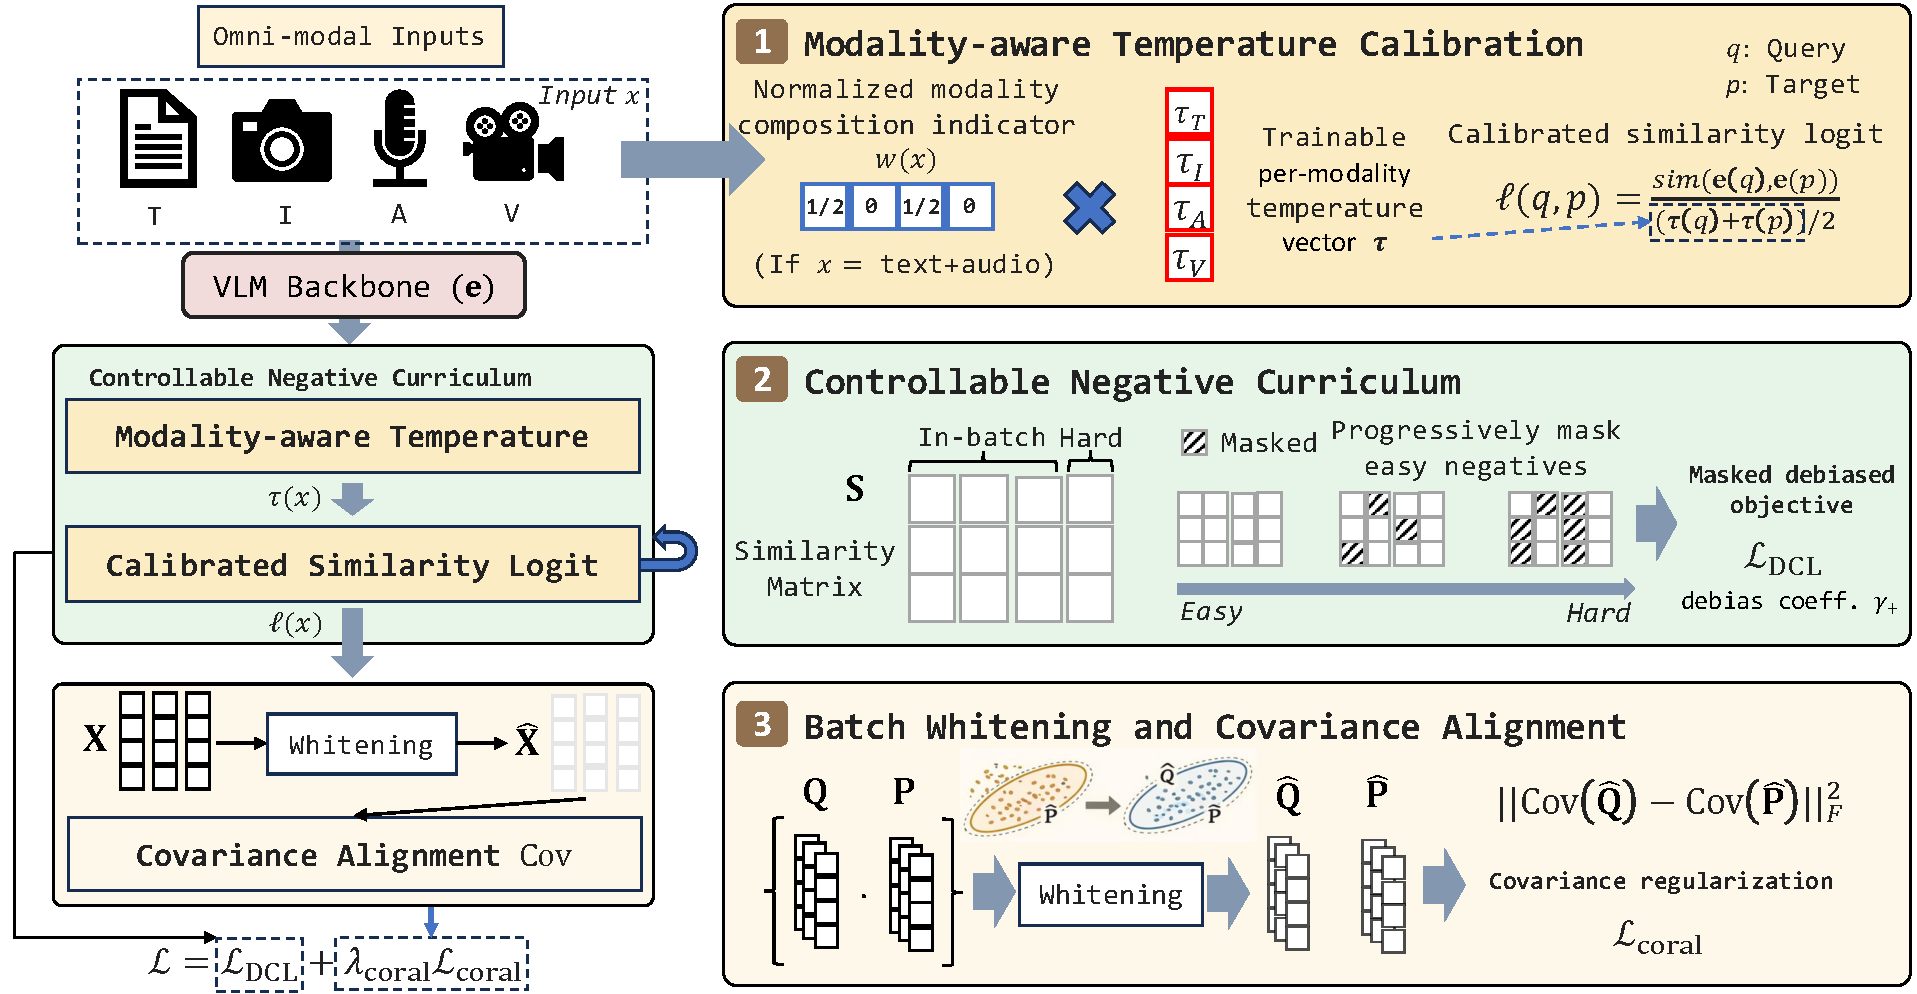
\includegraphics[width=0.98\textwidth]{figures/framwork.pdf}  
  \caption{\textbf{Overview of \ours{}.}
Given omni-modal inputs, \ours{} augments a VLM backbone with three lightweight components:
(1)~\textit{Modality-aware temperature calibration} computes a modality-composition indicator $w(x)$ and applies learnable modality-specific temperatures $\boldsymbol{\tau}$ to calibrate logits $\ell(q,p)$;
(2)~\textit{Controllable negative curriculum} progressively masks easy negatives and optimizes a masked debiased objective $\mathcal{L}_{\mathrm{DCL}}$;
(3)~\textit{Batch whitening and covariance alignment} whitens batch embeddings and adds a CORAL-style covariance regularizer.
}\label{fig:method_overview} 
\end{figure*}


In this section, we present \ours{}, a lightweight explicit-alignment framework that transforms a VLM into a unified omni-modal embedding model.
As shown in the left part of Fig.~\ref{fig:method_overview}, \ours{} preserves the backbone and introduces a simple training recipe.
Our framework comprises three components:
(1)~{Modality-aware temperature calibration}, which balances contrastive sharpness across modalities;
(2)~{A controllable negative curriculum}, which maintains a strong and stable learning signal; and
(3)~{Batch whitening and covariance alignment}, which harmonizes the shared-space geometry under heterogeneous inputs.
Together, these components improve the robustness of omni-modal embeddings without architectural modifications.



\subsection{Preliminaries}
We study omni-modal embedding with a base modality set
$\mathcal{M}_0=\{\texttt{T},\texttt{I},\texttt{A},\texttt{V}\}$,
corresponding to \emph{text}, \emph{image}, \emph{audio}, and \emph{video}.
Training data consist of tuples $(q, p^{+}, \mathcal{P}^{-})$,
where $q$ is a query, $p^{+}$ is its matched target, and $\mathcal{P}^{-}$ is a set of negative targets.
In this setting, $q$, $p^{+}$, and each $p^{-}\in\mathcal{P}^{-}$ can each take \emph{any} non-empty modality composition:
$
    q = x^{m_q}, p^{+}=x^{m_{+}}, p^{-}=x^{m_{-}}, \quad
    m_q,m_{+},m_{-}\in 2^{\mathcal{M}_0}\setminus\{\emptyset\}
$, where we denote an input with modality composition $m$ as $x^{m}$.

We consider two common sources of negatives: (i)~\textbf{in-batch negatives}, \eg, other positive targets in the same mini-batch, and
(ii)~\textbf{hard negatives}, mined by a retriever or constructed via heuristics.

Our objective is to learn a single embedding function $ \mathbf{e}(\cdot): \ \mathcal{X} \rightarrow \mathbb{R}^{D}, $
where $\mathcal{X}$ denotes the space of omni-modal inputs.
The embedding maps any omni-modal input into a shared representation space,
so that matched pairs $(q,p^{+})$ are close while mismatched pairs $(q,p^{-})$ are well separated.




\subsection{Modality-aware Temperature Calibration}
\label{subsec:method-modaltemp}

A single global temperature in contrastive learning implicitly assumes that all inputs induce similarity logits with comparable sharpness~\cite{simclr}.
In the omni-modal setting, different modalities can exhibit very different levels of ambiguity and noise.
As a result, a fixed temperature can make some modality compositions overly sharp while leaving others overly flat, leading to imbalanced gradients and unstable optimization.

To address this issue, we introduce a lightweight modality-aware temperature module implemented as a learnable per-modality scaling vector
$\boldsymbol{\tau}\in\mathbb{R}^{|\mathcal{M}_0|}$.
As shown in the top right part of Fig.~\ref{fig:method_overview}, for any input $x$, we construct a normalized modality-indicator weight
$w(x)\in\Delta^{|\mathcal{M}_0|-1}$ based on its modality composition.
Concretely, $w(x)$ assigns non-zero mass to every modality present in $x$ and is normalized by the number of active modalities.
We then define an \emph{instance temperature} as a weighted sum
$
\tau(x)=\max\!\big(w(x)^{\top}\boldsymbol{\tau},\,10^{-6}\big).
$
Given any pair $(q,p)$, we use a symmetric pairwise temperature
$
\tau(q,p)=\left(\tau(q)+\tau(p)\right)/2,
$
and compute the calibrated similarity logit as
\begin{equation}
\ell(q,p)=\frac{\mathrm{sim}(\mathbf{e}(q),\,\mathbf{e}(p))}{\tau(q,p)}\,.
\end{equation}
We use $\ell(\bullet,\bullet)$ consistently in the contrastive learning objective.


Intuitively, larger $\tau$ flattens logits while smaller $\tau$ sharpens logits, so noisier/ambiguous modalities tend to learn larger temperatures.
This stabilizes contrastive gradients in mixed omni-modal batches.




\subsection{Controllable Negative Curriculum}
\label{subsec:method-hns}
In omni-modal contrastive training, the hardness of negatives varies widely across batches and modalities, causing either weak supervision (overly easy negatives) or unstable optimization (false negatives).
To address this \emph{hardness imbalance}, we adopt a simple curriculum that gradually increases the focus on confusing negatives.
However, hard-negative selection is prone to \emph{selection bias}, since the hardest samples often include near-duplicates or semantically related items (\ie, false negatives), which can destabilize learning.
As shown in the middle right of Fig.~\ref{fig:method_overview}, we therefore combine negative selection with Debiased Contrastive Learning (DCL)~\cite{dcl}, which down-weights the aggregated negative to reduce the impact of potential false negatives.


For a mini-batch $\mathcal{B}=\{(q_i,p_i^{+},\mathcal{P}_i^{-})\}_{i=1}^{B}$, we form a similarity matrix
$\mathbf{S}\in\mathbb{R}^{B\times(B+K)}$, where the first $B$ columns correspond to the in-batch paired targets $\{p_j^{+}\}_{j=1}^{B}$, \ie, in-batch negatives
($S_{ij}=\ell(q_i,p_j^{+})$), and the remaining $K$ columns correspond to mined hard negatives
($S_{i,B+k}=\ell(q_i,p_{i,k}^{-})$). 
The diagonal $S_{ii}$ is the positive for row $i$.
We then mask negatives by keeping only the top fraction of the most confusing items per row.
Concretely, at training step $t$ we use a quantile threshold $\rho_t\in[0,1)$ and keep the hardest
$(1-\rho_t)$ fraction among all negatives in each row: for each $i$, let $\mathcal{N}_i(\rho_t)$ be the
set of indices of the largest $k=\lfloor(1-\rho_t)(B+K-1)\rfloor$ values in $\{S_{ij}\}_{j\neq i}$.
This produces a boolean mask $\mathbf{M}\in\{0,1\}^{B\times(B+K)}$ where $M_{ij}=1$ iff $j\in\mathcal{N}_i(\rho_t)$
(and $M_{ii}=0)$.

\paragraph{Masked DCL objective.}
We apply the mask inside a DCL loss by summing only over selected negatives.
Let $\Omega_i=\{i\}\cup \mathcal{N}_i(\rho_t)$.
DCL corrects the bias of (masked) negative sampling by subtracting a scaled positive term from the negative aggregate:
\begin{equation}
\mathcal{L}_{\mathrm{DCL}}
=-\frac{1}{B}\sum_{i=1}^{B}\log
\frac{\exp(S_{ii})}{\exp(S_{ii})+\widetilde{N}_i}\,,
\label{eq:dcl}
\end{equation}
$$
\widetilde{N}_i=\max\!\Big(\sum_{j\in\Omega_i\setminus\{i\}} \exp(S_{ij})-\gamma_{+}\exp(S_{ii}),\,\epsilon\Big)\,,
$$
where $\gamma_{+}\in(0,1)$ is the debiasing coefficient and $\epsilon$ is a small constant for numerical stability.
Here $\mathbf{S}$ is computed from the calibrated logit $\ell(\bullet,\bullet)$, hence no extra global temperature is required.


\paragraph{Curriculum schedule.}
Recall that $\rho_t$ denotes the \emph{mask ratio} of negatives, so a larger $\rho_t$ means fewer negatives are kept (and the remaining set is harder).
We therefore start with a smaller $\rho_t$ (keeping a larger fraction of negatives, including easier ones), and linearly increase it after a warmup period to gradually focus on fewer, harder negatives:
$$
\rho_t=\rho_{\mathrm{init}}+(\rho_{\mathrm{final}}-\rho_{\mathrm{init}})\,
\mathrm{clip}\!\left(\frac{t-t_0}{T-t_0},\,0,\,1\right),
$$
where $t$ is the training step, $t_0$ is the warmup cutoff (the step after which we start increasing $\rho_t$, i.e., hardness), $T$ is the total number of training steps, and $\mathrm{clip}(x,0,1)=\min(\max(x,0),1)$.


This curriculum lets the model first learn coarse omni-modal alignment with stable gradients, and then progressively resolve fine-grained confusions with genuinely hard negatives, while DCL mitigates the bias amplified by negative selection---together yielding stable optimization and cleaner alignment under mixed-modality batches.



\begin{table*}[t]
\centering
\caption{Overall results on MMEB-V2, which contains \textbf{78 tasks} spanning three major groups: \textbf{Image} (36 tasks), \textbf{Video} (18 tasks), and \textbf{VisDoc} (24 visual document tasks). 
We report group-wise averages and the overall score across all tasks.
We group prior baselines by their supported modality sets (\textit{bi-modal}, \textit{tri-modal}, and \textit{omni-modal}) and additionally report \ours{} w/o.\ explicit alignment (vanilla contrastive) as a strong baseline.
We highlight the best score in \textbf{bold} and the second-best with an \underline{underline}.
``$\dag$'' denotes our model outperforms all baselines significantly in paired t-test at $p<0.01$ level (with Bonferroni correction).
}\label{tab:mmeb-v2-overall}
%\setlength{\tabcolsep}{6.0pt}
%\setlength{\extrarowheight}{1.1pt}
\begin{tabular}{l c cccc}
\toprule
Model & Size & Image & Video & VisDoc & All \\
\midrule
\multicolumn{6}{l}{\textit{Text + Image (Bi-modal)}} \\
ColPali-v1.3~\cite{ColPali}        & 3B & 34.9 & 28.2   & 71.0   & 44.4 \\
VLM2Vec-v1~\cite{MMEB}       & 7B   & 65.5 & 33.7 & 46.4 & 52.3 \\
GME~\cite{GME}            & 7B   & 56.0 &	38.4 & {75.2} & 57.8 \\
CAFe~\cite{CAFe}      & 7B & 67.6 & 42.4   & 63.9   & 60.6 \\
\midrule
\multicolumn{6}{l}{\textit{Text + Image + Video}} \\
VLM2Vec-v2~\cite{MMEB-v2}       & 2B  & 64.9	& 34.6	& 65.4	& 58.0 \\
UniME-V2~\cite{UniME-V2}             & 7B  & {71.8}	& 39.0	& 56.7	& 59.6 \\
UME-R1~\cite{UME-R1}                 & 7B  & 71.3	& {47.5}	& 67.1	& \underline{64.5} \\
\midrule
\multicolumn{6}{l}{\textit{Text + Image + Video + Audio (Omni-modal)}} \\
Tevatron-Omni~\cite{tevatron-omni}   & 7B  & 37.1	& 35.1	& 74.5	& 48.1 \\
LCO-EMB~\cite{LCO-Embed}   & 7B  & 44.0 & 	38.2	& 69.8	& 50.6 \\
Omni-Embed-Nemotron~\cite{Nemotron}  & 3B  & 43.7	& 36.9	& 74.2	& 51.5 \\
\midrule
\multicolumn{6}{l}{\textit{Ours w/o. explicit alignment (vanilla contrastive)}} \\
\ours{}-vanilla-3B & 3B & 65.8 & 39.3 & 72.0 & 62.0 \\
\ours{}-vanilla-7B & 7B & 69.0 & 41.8 & 74.7 & 64.4 \\
\midrule
\multicolumn{6}{l}{\textit{Ours (Omni-modal)}} \\
\ours{}-3B & 3B & 67.6 & 40.6 & 73.2 & 63.1 \\
\ours{}-7B & 7B & 71.2 & 43.5 & 76.1 & \textbf{66.4}$^\dag$ \\
\bottomrule
\end{tabular}
\vspace{-0.12cm}
\end{table*}


\subsection{Batch Whitening and Covariance Alignment}
\label{subsec:method-align}

Representations produced by an omni-modal backbone often exhibit mismatched second-order statistics, which can distort similarity geometry and destabilize ranking~\cite{DBLP:journals/corr/abs-2103-15316}, especially when batches mix diverse modality compositions.
To explicitly regularize the shared embedding space, we apply batch whitening~\cite{Whiten} and add a CORAL-style covariance alignment loss~\cite{coral} as a regularizer.

For a mini-batch $\mathcal{B}=\{(q_i,p_i^{+},\mathcal{P}_i^{-})\}_{i=1}^{B}$, we compute embeddings with the shared encoder $\mathbf{e}(\cdot)$ and stack them as
$
\mathbf{Q}=[\mathbf{e}(q_i)]_{i=1}^{B}\in\mathbb{R}^{B\times D},
\mathbf{P}=[\mathbf{e}(p_i^{+})]_{i=1}^{B}\in\mathbb{R}^{B\times D}.
$
We compute a single whitening transform $W$ from the concatenation of query and target embeddings in the mini-batch, and apply the same transform to both sets:
$\widehat{\mathbf{Q}}=W(\mathbf{Q})$ and $\widehat{\mathbf{P}}=W(\mathbf{P})$.
We then define the empirical covariance operator for any batch embedding matrix $\mathbf{X}\in\mathbb{R}^{B\times D}$ (\eg, $\widehat{\mathbf{Q}}$ or $\widehat{\mathbf{P}}$) as
\begin{equation}
\mathrm{Cov}(\mathbf{X})=\frac{1}{B-1}(\mathbf{X}-\bar{\mathbf{X}})^{\top}(\mathbf{X}-\bar{\mathbf{X}})\,\,,
\label{eq:cov}
\end{equation}
where $\bar{\mathbf{X}}$ is the feature-wise mean over the batch.
The CORAL loss is
\begin{equation}
\mathcal{L}_{\mathrm{coral}}
=\frac{1}{4D^{2}}
\left\|
\mathrm{Cov}(\widehat{\mathbf{Q}})-\mathrm{Cov}(\widehat{\mathbf{P}})
\right\|_{F}^{2}.
\label{eq:coral_loss}
\end{equation}
With Eq.(\ref{eq:dcl}) and Eq.(\ref{eq:coral_loss}), the final objective is
\begin{equation}
\mathcal{L}
=\mathcal{L}_{\mathrm{DCL}}+\lambda_{\mathrm{coral}}\mathcal{L}_{\mathrm{coral}}\,\,,
\end{equation}
where $\lambda_{\mathrm{coral}}$ controls the strength of covariance regularization.
In practice, we implement $W(\cdot)$ with a numerically stable routine (\eg, group-wise computation with a small jitter) to avoid instability under high-dimensional embeddings.
By reducing second-order mismatch between $\widehat{\mathbf{Q}}$ and $\widehat{\mathbf{P}}$, this regularizer improves geometric consistency in the shared space and stabilizes similarity-based ranking in omni-modal retrieval.




